% Latex template: mahmoud.s.fahmy@students.kasralainy.edu.eg
% For more details: https://www.sharelatex.com/learn/Beamer

\documentclass{beamer}					% Document class
    \usepackage[T2A]{fontenc}			% кодировка
    \usepackage[utf8]{inputenc}			% кодировка исходного текста
    \usepackage[english,russian]{babel}				% Set language
    % \usepackage[utf8x]{inputenc}			% Set encoding
    \mode<presentation>						% Set options
    {
      \usetheme{default}					% Set theme
      \usecolortheme{default} 				% Set colors
      \usefonttheme{default}  				% Set font theme
      \setbeamertemplate{caption}[numbered]	% Set caption to be numbered
    }
    
    \usepackage{graphicx}					% For including figures
    \usepackage{booktabs}					% For table rules
    \usepackage{hyperref}					% For cross-referencing
    
    \usepackage{amsmath} % some math-related packages, not sure which of them are necessary
    \usepackage{amssymb}
    \usepackage{amsfonts}
    \usepackage{bm}
    \usepackage{fixmath} % for \mathbold

    \AtBeginSection[]{
        \begin{frame}
        \vfill
        \centering
        \begin{beamercolorbox}[sep=8pt,center,shadow=true,rounded=true]{title}
          \usebeamerfont{title}\insertsectionhead\par%
        \end{beamercolorbox}
        \vfill
        \end{frame}
      }
    



    \title{Дифференцируемая нижняя граница для математического ожидания метрики \color{blue}{BLEU}}	% Presentation title
    \author{
        Студент: Жуков В.А. МФТИ ФИВТ, 4 курс
        \vfill
        Научный руководитель: Кретов М.К.
    }			
    % \author[shortname]{author1  \and author2 }
    % \institute[shortinst]{\inst{1} asd for author1 \and %
    %                   \inst{2} affiliation for author2}
    % Presentation author								% Today's date	
    \date{25 Июня 2018}
    \begin{document}
    
    % Title page
    % This page includes the informations defined earlier including title, author/s, affiliation/s and the date
    \begin{frame}
      \titlepage
    \end{frame}
    
    % Outline
    % This page includes the outline (Table of content) of the presentation. All sections and subsections will appear in the outline by default.
    \begin{frame}{Содержание}
      \tableofcontents
    \end{frame}
    
    % The following is the most frequently used slide types in beamer
    % The slide structure is as follows:
    %
    %\begin{frame}{<slide-title>}
    %	<content>
    %\end{frame}
    
    \section{Введение и основные понятия}
    
    \begin{frame}{Машинный перевод}
        Подходы к задаче машинного перевода:
        \begin{itemize}
            \item Статистический машинный перевод (SMT)
            \item \color{blue}{Нейронный машинный перевод (NMT)}
        \end{itemize}
    \end{frame}
    

    \begin{frame}{Оценка качества}
        Метрики качества в задаче машинного перевода:
        \begin{itemize}
            \item {\color{blue}{BLEU}}
            \item ROUGE
            \item METEOR
        \end{itemize}
    \end{frame}

    \begin{frame}{Sequence to sequence архитектура}
        \begin{figure}
            \centering
            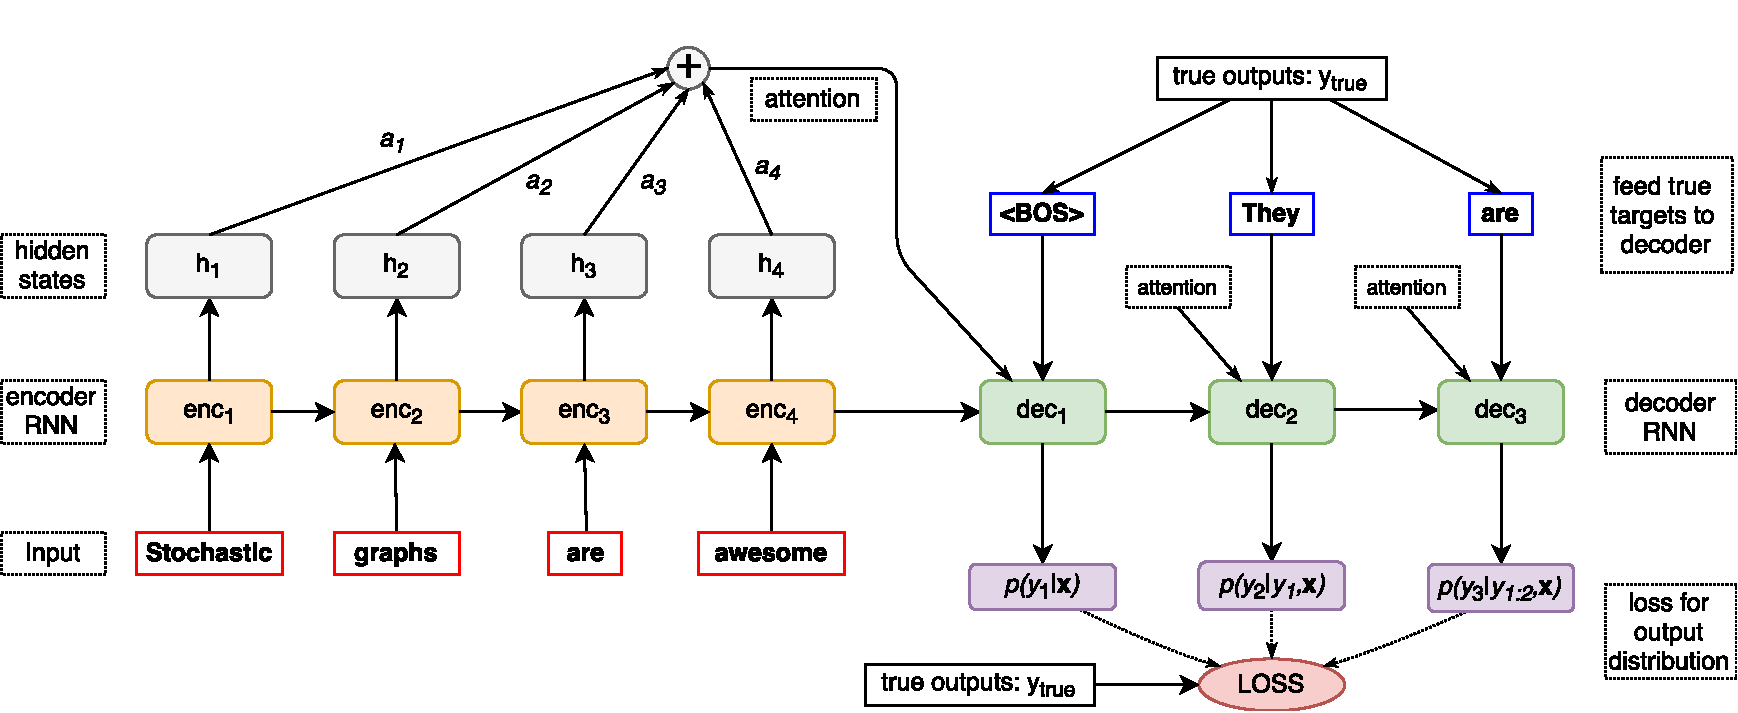
\includegraphics[width=1.0\linewidth]{seq2seq.pdf}
            \caption{Пример модели seq2seq с механизмом внимания; фаза обучения}
            \label{fig:seq2seq}
        \end{figure}
    \end{frame}

     \begin{frame}{Общий подход к оптимизации произвольной метрики}
        \begin{block}{Правило REINFORCE}
        $$ \nabla_\theta \mathbb{E}_{p(z;\theta)}[f(z)] = \mathbb{E}_{p(z;\theta)}[f(z)\nabla_\theta \log p(z;\theta)] $$
        $ p(z; \theta) $ -- функция правдоподобия

        $ f(z) $ -- оптимизируемая функция
        \end{block}
    \end{frame}

    % \begin{frame}{Стохастические вычислительные графы}
    %     \begin{equation*}
    %         \mathbb{E}_{v \in S}\Bigg[\underbrace{\sum_{w \in \mathcal{S}, \theta \prec^D w} \left(
    %         \frac{\partial}{\partial \theta} \log p(w|\textrm{DEPS}_w)
    %         \right) \sum_{c \in \mathcal{C}, w \prec c} \hat{c}}_{\textrm{(A)}} + 
    %     \end{equation*}
    %     $$
    %     \underbrace{\sum_{c \in \mathcal{C}, \theta \prec^D c} \frac{\partial}{\partial \theta}
    %         c(\textrm{DEPS}_c)}_{\textrm{(B)}}\Bigg].
    %     $$
    % \end{frame}
    \section{Цель работы}
    \begin{frame}{Цель работы}
        Предложить более эффективный способ оптимизации (в сравнении с REINFORCE) для метрики BLEU.
        \vfill
        \begin{equation}
            \mathbb{E}_{\mathrm{data}} \mathbb{E}_{\mathrm{arch\_stoch}}  \color{blue}{\mathbb{E}_{\mathrm{output}} \textnormal{BLEU}(x, y) \to \max} 
        \end{equation}
    \end{frame}

    \section{Предлагаемый метод}
    \subsection{Постановка задачи и используемые обозначения}
    \begin{frame}{Метрика BLEU}
        \begin{equation}
            {\color{blue}{\textrm{BLEU}}=\textrm{BP} \cdot \exp \left(\sum\limits_{n=1}^N{w_n \log p_n}\right)}
        \end{equation}
        Обычно $w_n = 1/N, N = 4$.
        \vfill
        \begin{equation}
            \textrm{BP} =
            \begin{cases}
            1 & \text{if}\ c>r \\
            e^{1 - r/c} & c \le r
            \end{cases}
        \end{equation}
    \end{frame}

    \begin{frame}{Нижняя граница}
        \begin{block}{План вывода}
        \begin{itemize}
            \item Записать метрику {\color{blue}{BLEU}} в матричном виде.
            \item Обозначить предположения необходимые для вывода.
            \item Вывод оценки.
        \end{itemize}
        \end{block}
    \end{frame}

    \subsection{Вывод нижней границы}

    % \begin{frame}{Нижняя граница}
    %     R = "Петя взял яблоко,  яблоко оказалось вкусным"

    %     C = "Яблоко"
    %     \begin{block}{модифицированные точности}
    %     \begin{equation}
    %         p_n \sim O_n
    %         \label{p_n}
    %     \end{equation}

    %     \begin{equation}
    %         O_n = \sum\limits_{\textnormal{n-gram} \in C} \textnormal{min(Count$_C$(n-gram), Count$_R$(n-gram))}
    %         \label{Oprime}
    %     \end{equation}
    %     \end{block}
    %     $$O_1 = \min(\textrm{Count}_C(\textrm{яблоко}), \textrm{Count}_R(\textrm{яблоко})) = \min(1, 2) = 1$$
    % \end{frame}

    \begin{frame}{Нижняя граница}
        \begin{block}{Представление BLEU в матричном виде}
            матрица x $[\textrm{len}_C \times v]$
            
            матрица $y$ $[\textrm{len}_R \times v]$
            

            \begin{equation}
                \textnormal{{\color{blue}{BLEU(C, R)}}} = function(x, y)
            \end{equation}   
        \end{block}       
          
    \end{frame}

    \begin{frame}{Нижняя граница}
        \begin{block}{Необходимые предположения}
            \begin{itemize}
            \item Матрица $p_x$ получена детерминистически
            \item Слова $R$ уникальны.
            \end{itemize}
        \end{block}       
        
    \end{frame}

    \begin{frame}{Нижняя граница}
        \begin{block}{Итог вывода}
        Выход модели $p_x$  $[seq\_len \times vocab\_size]$\\
        Метки тренировочной выборки $p_y$  $[seq\_len \times vocab\_size]$.
        $$\mathbb{E}_{\mathrm{output} = x \sim p_x} \textnormal{{\color{blue}{BLEU(x, y)}}} \ge function(p_x, p_y) := \textnormal{\color{blue}{LB}}$$
        \end{block}
    \end{frame}

    \section{Эксперименты и результаты}
    \subsection{Модельная задача}
    \begin{frame}{Модельная задача}
        \begin{itemize}
         \item   Размер словаря равен 10000

         \item   Последовательности длины 10

         \item   Матрица $p_x$ сгенерированная случайно

         \item  Функция потерь {\color{blue}{LB}}

         \item   Оптимизируется матрица $p_x$

        \end{itemize}
    \end{frame}

    \begin{frame}{Модельная задача}
        \begin{figure}[h]
            \centering
            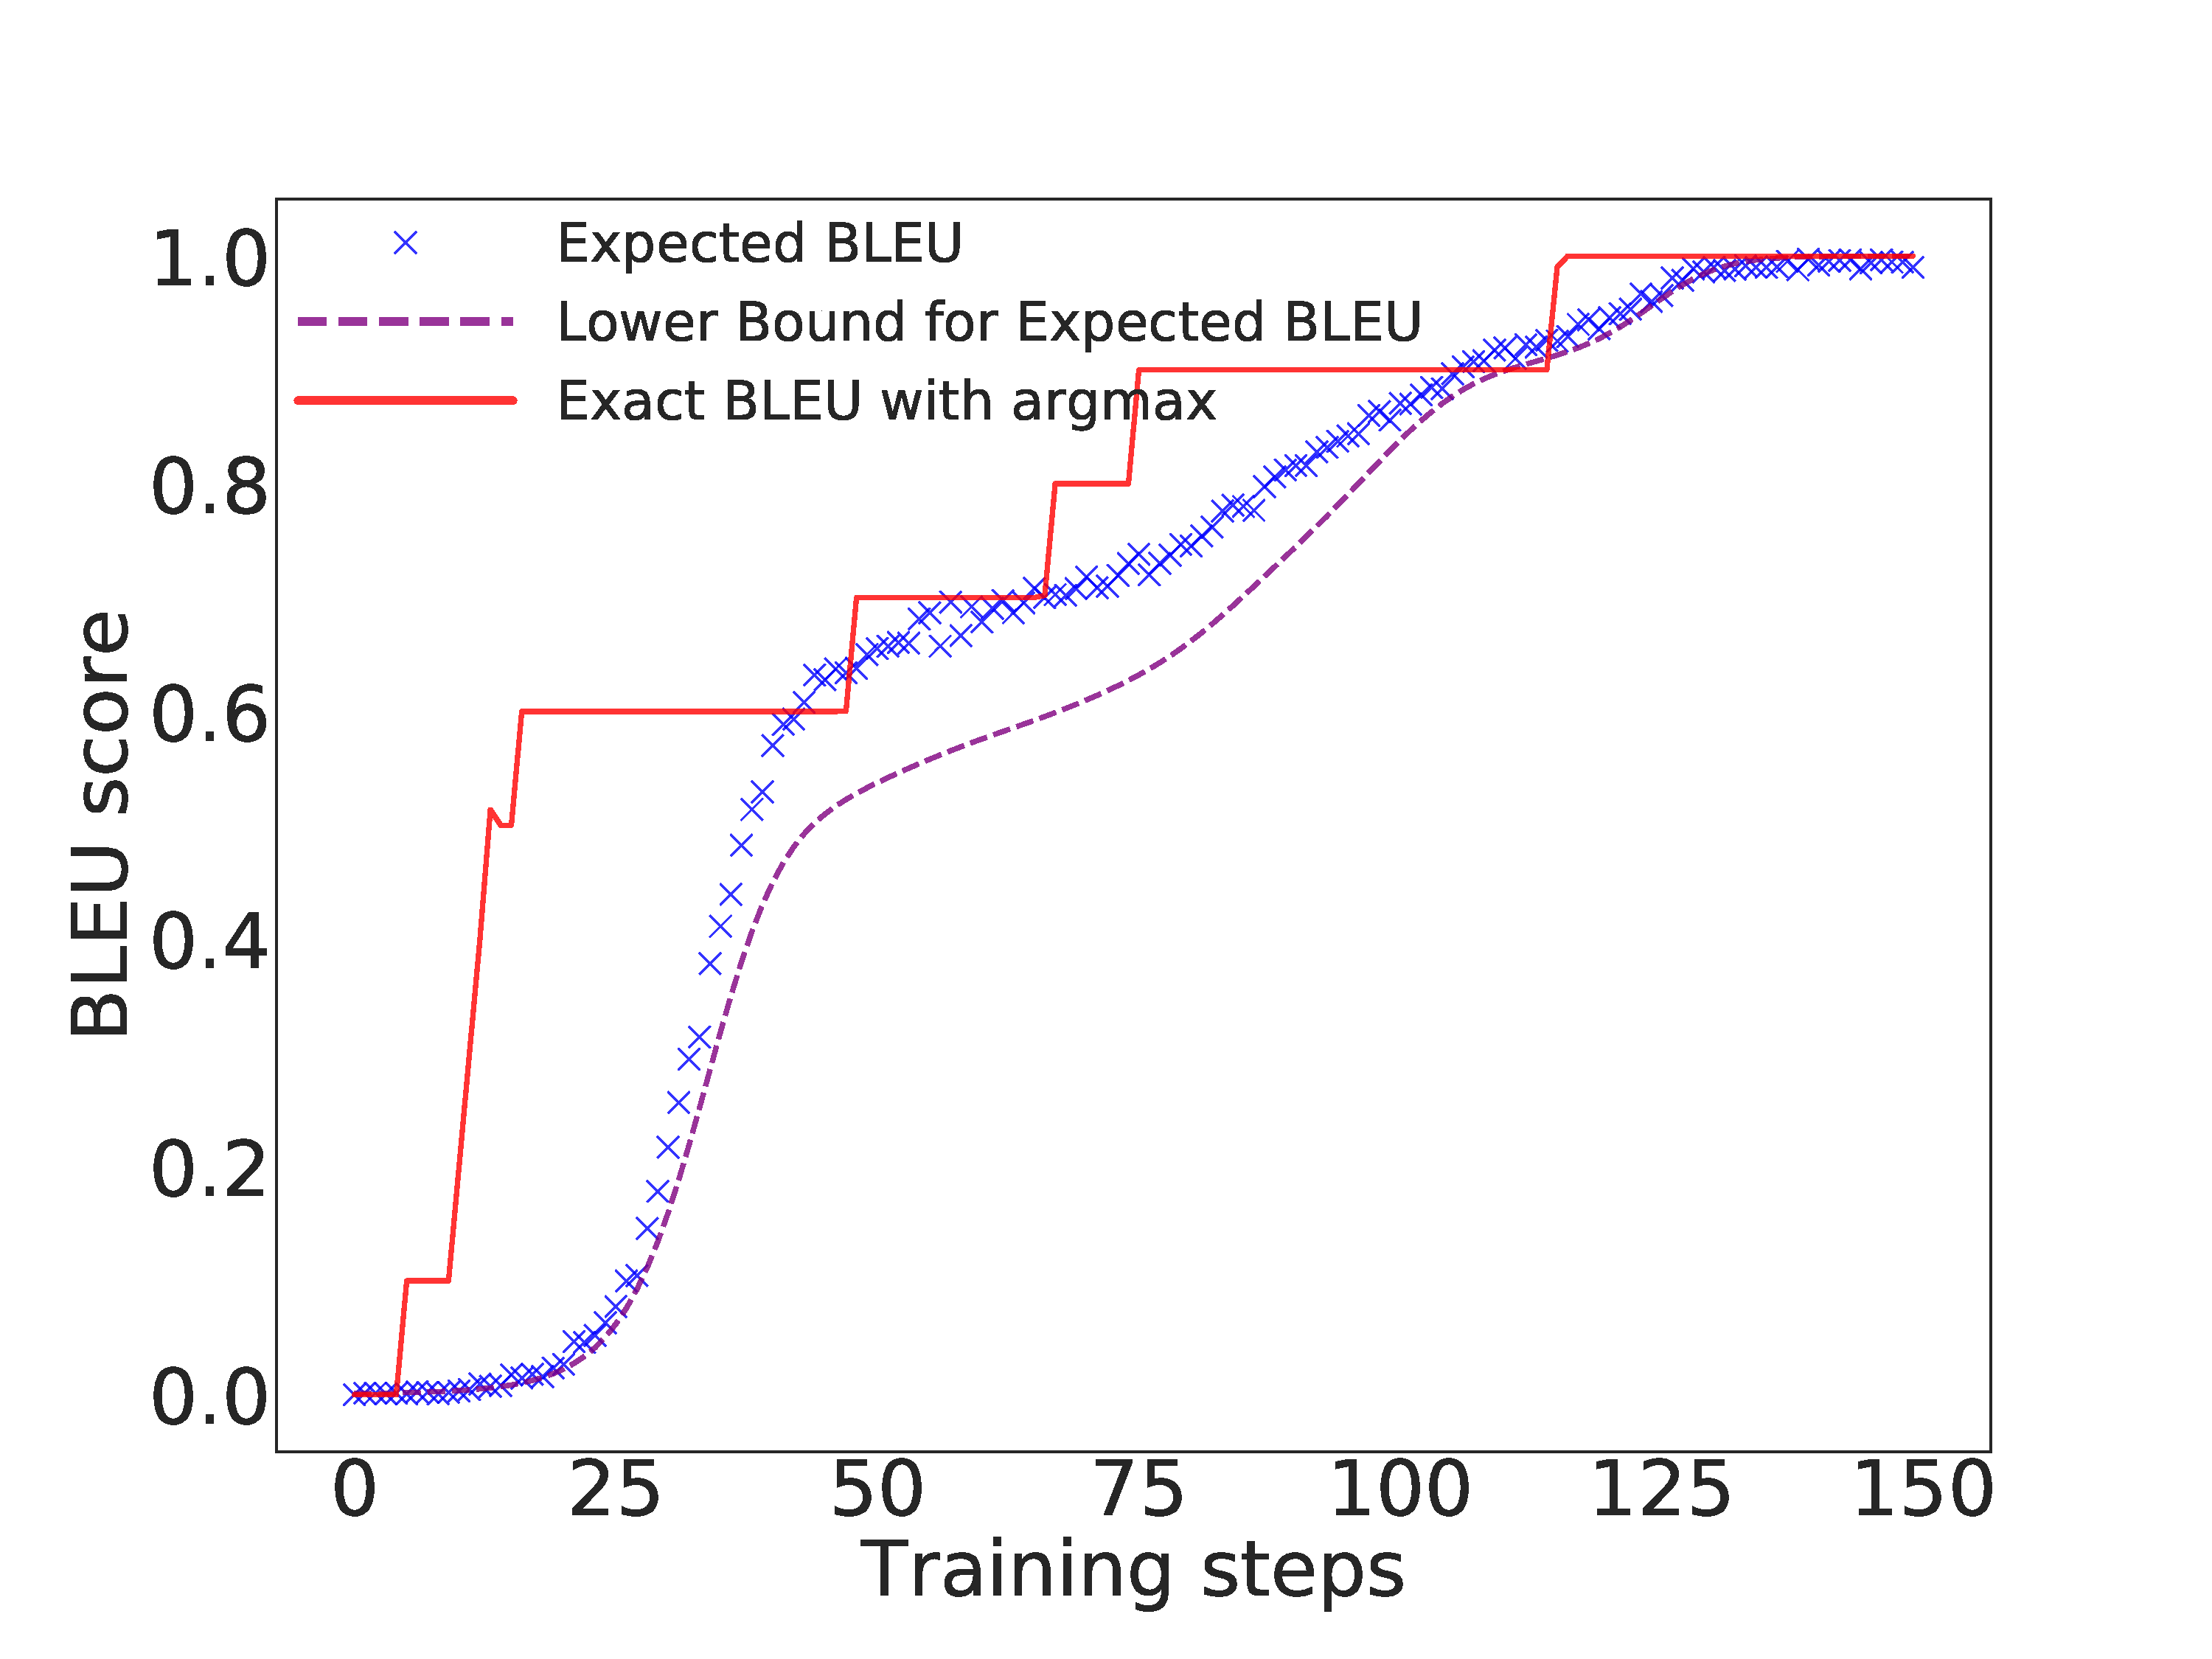
\includegraphics[scale=0.2]{BLEU_old.pdf}
            \label{fig:bleu_toy}
        \end{figure}
    \end{frame}
      
    \begin{frame}{Модельная задача}
        \begin{figure}[h]
            \centering
            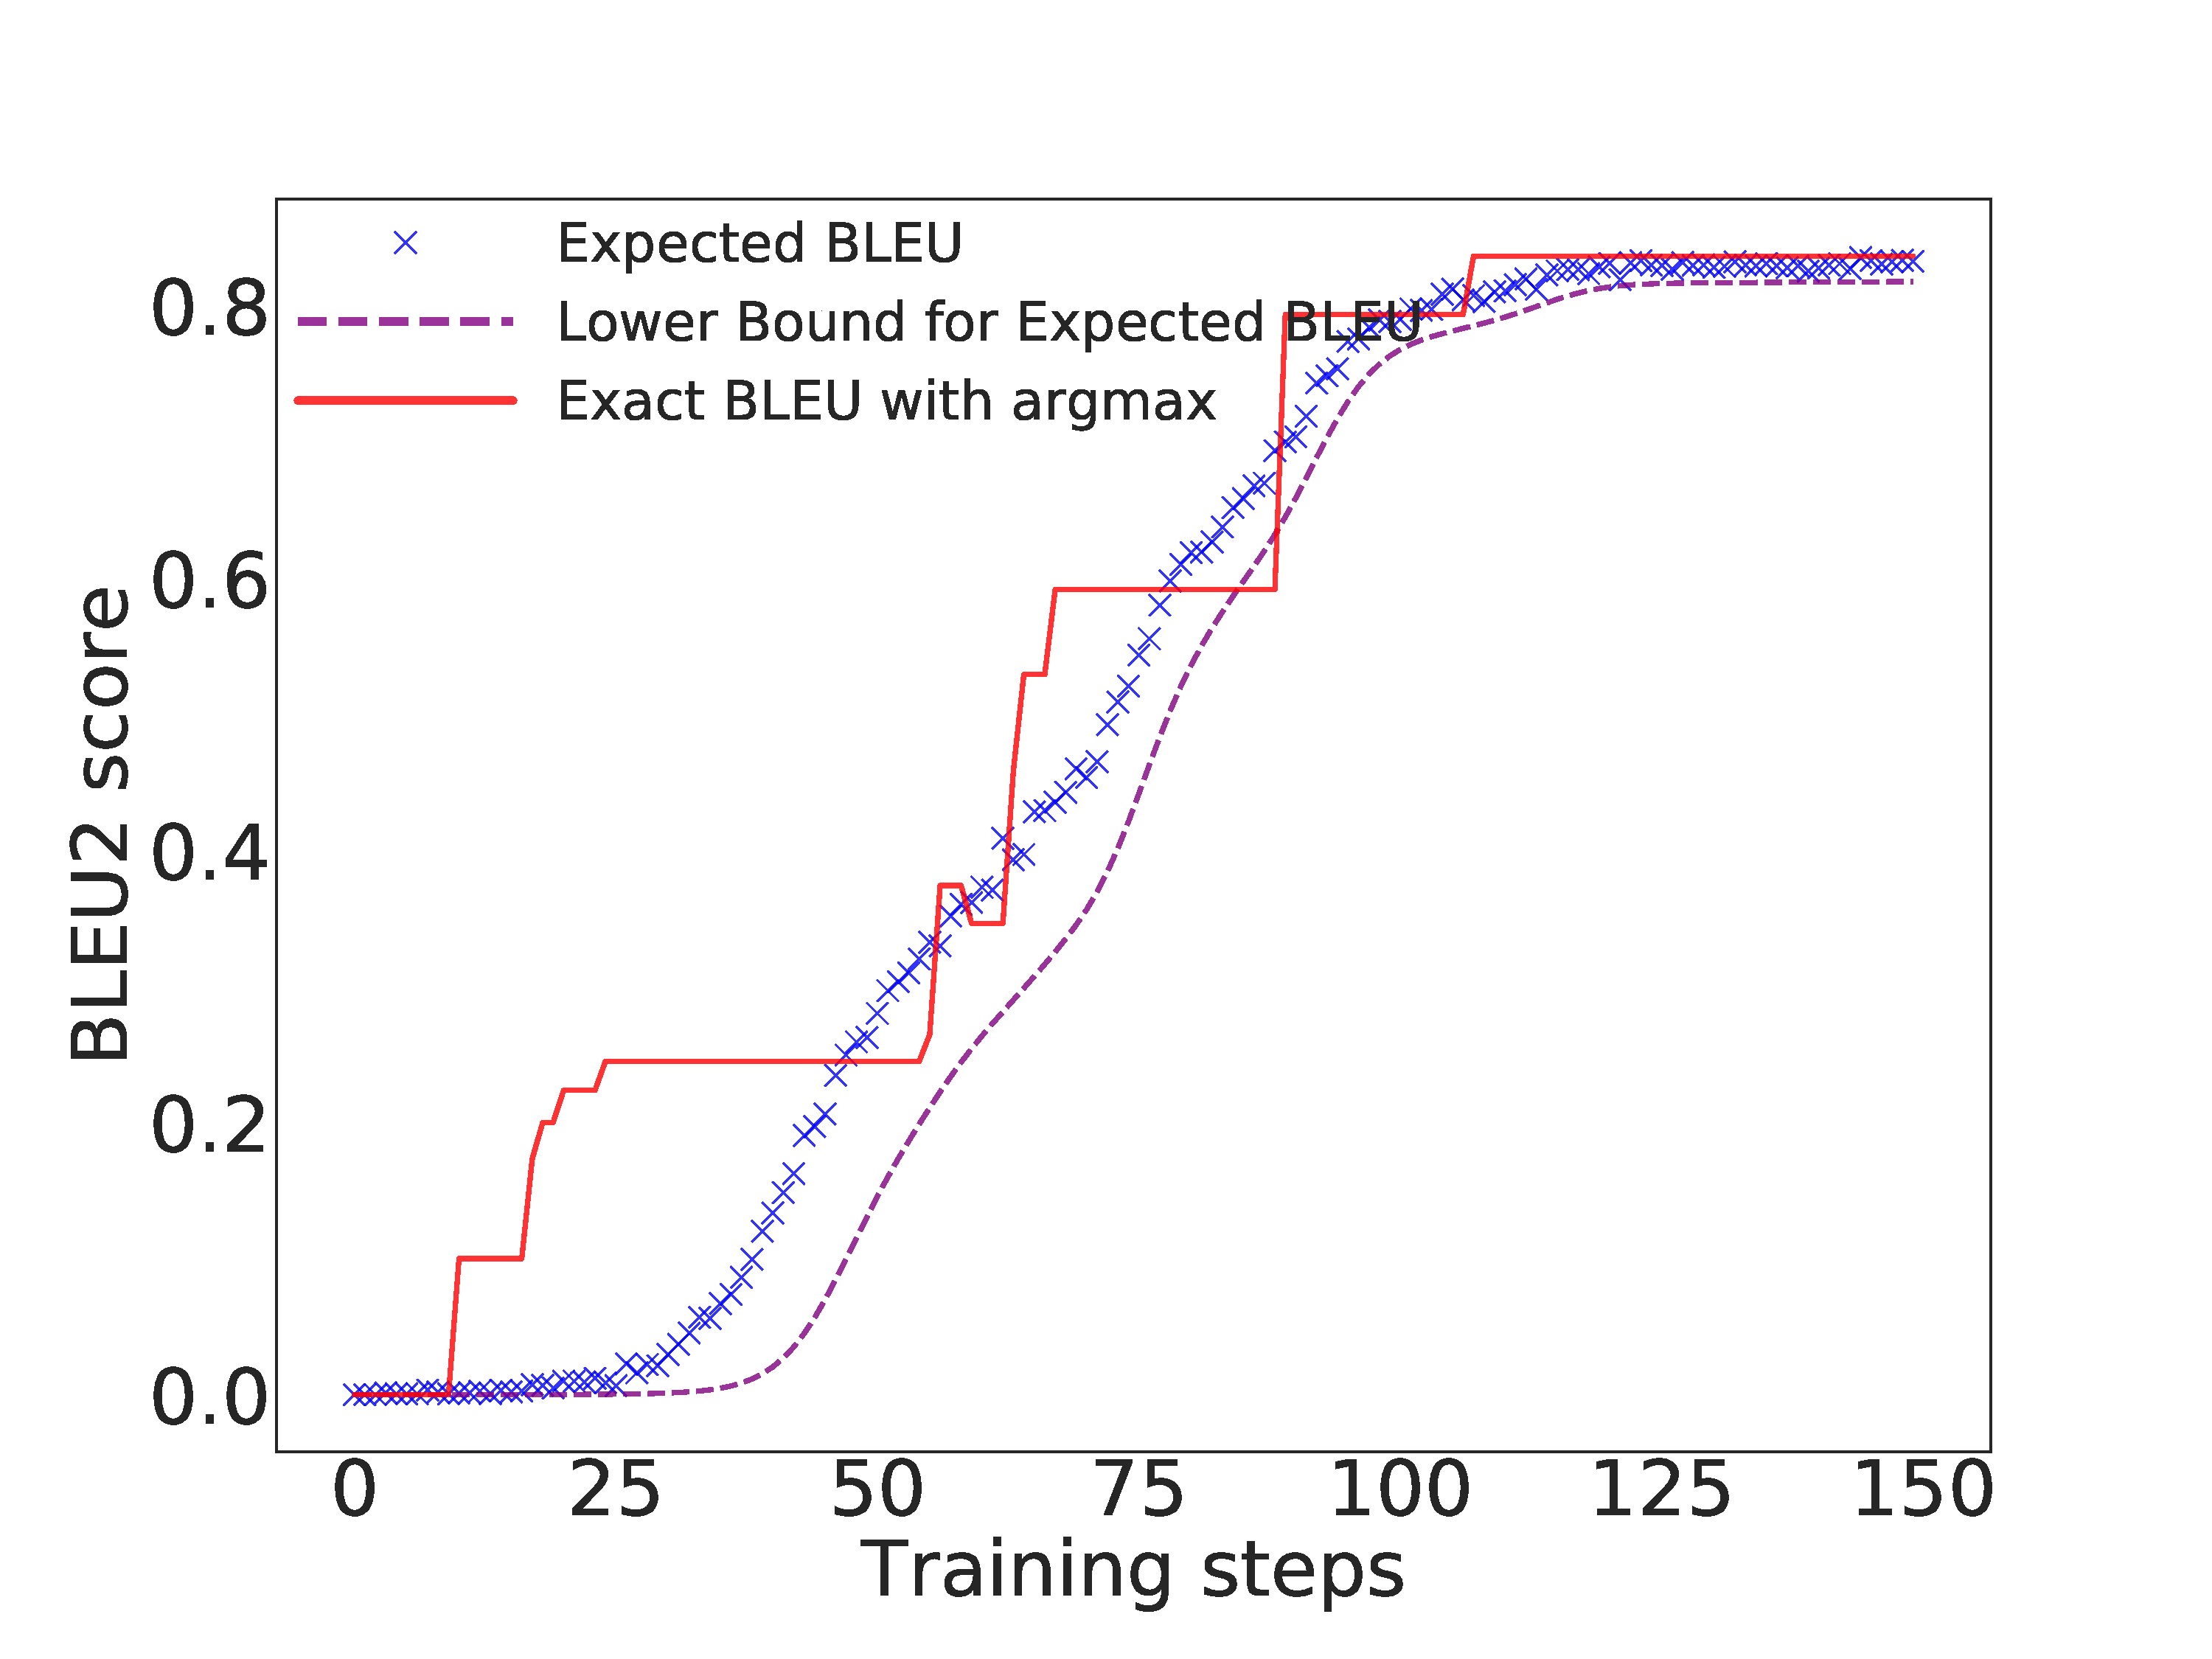
\includegraphics[scale=0.2]{BLEU2_old.pdf}
            \label{fig:bleu2_toy}
        \end{figure}
    \end{frame}

    \subsection{Задача машинного перевод}
    \begin{frame}{Результаты на задаче машинного перевода}
        \begin{table}[t!]
            \begin{center}
            \begin{tabular}{|l|ccc|}
            \hline \bf & \bf CE & \bf RF & \bf LB \\ \hline
            1&$26.60\pm 0.14$&$27.16\pm 0.18$&$\textbf{27.83}\pm\textbf{0.17}$\\
            5&$27.56\pm 0.17$&$27.85\pm 0.11$&$\textbf{28.10}\pm\textbf{0.17}$\\
            \hline
            \end{tabular}
            \end{center}
            \caption{\label{results_translation_IWSLT} Результат на задаче перевода для датасета IWSLT'14. 
            
            DE $\to$ EN}
            \end{table}
    \end{frame}


    \begin{frame}{Результаты на задаче перевода}
        \begin{table}[t!]
        \begin{center}
        \begin{tabular}{|l|cc|}
        \hline \bf & \bf CE & \bf LB \\ \hline
        1&$17.12\pm 0.2$&$\textbf{18.65}\pm\textbf{0.13}$\\
        5&$\textbf{19.23}\pm \textbf{0.19}$&$19.03\pm 0.15$\\
        \hline
        \end{tabular}
        \end{center}
        \caption{\label{results_translation_WMT} Результат на задаче перевода для датасета WMT'14. 
        
        EN $\to$ DE}
        \end{table}
    \end{frame}
    \begin{frame}{Результаты на задаче перевода}
        \begin{figure}[h]
        \centering
        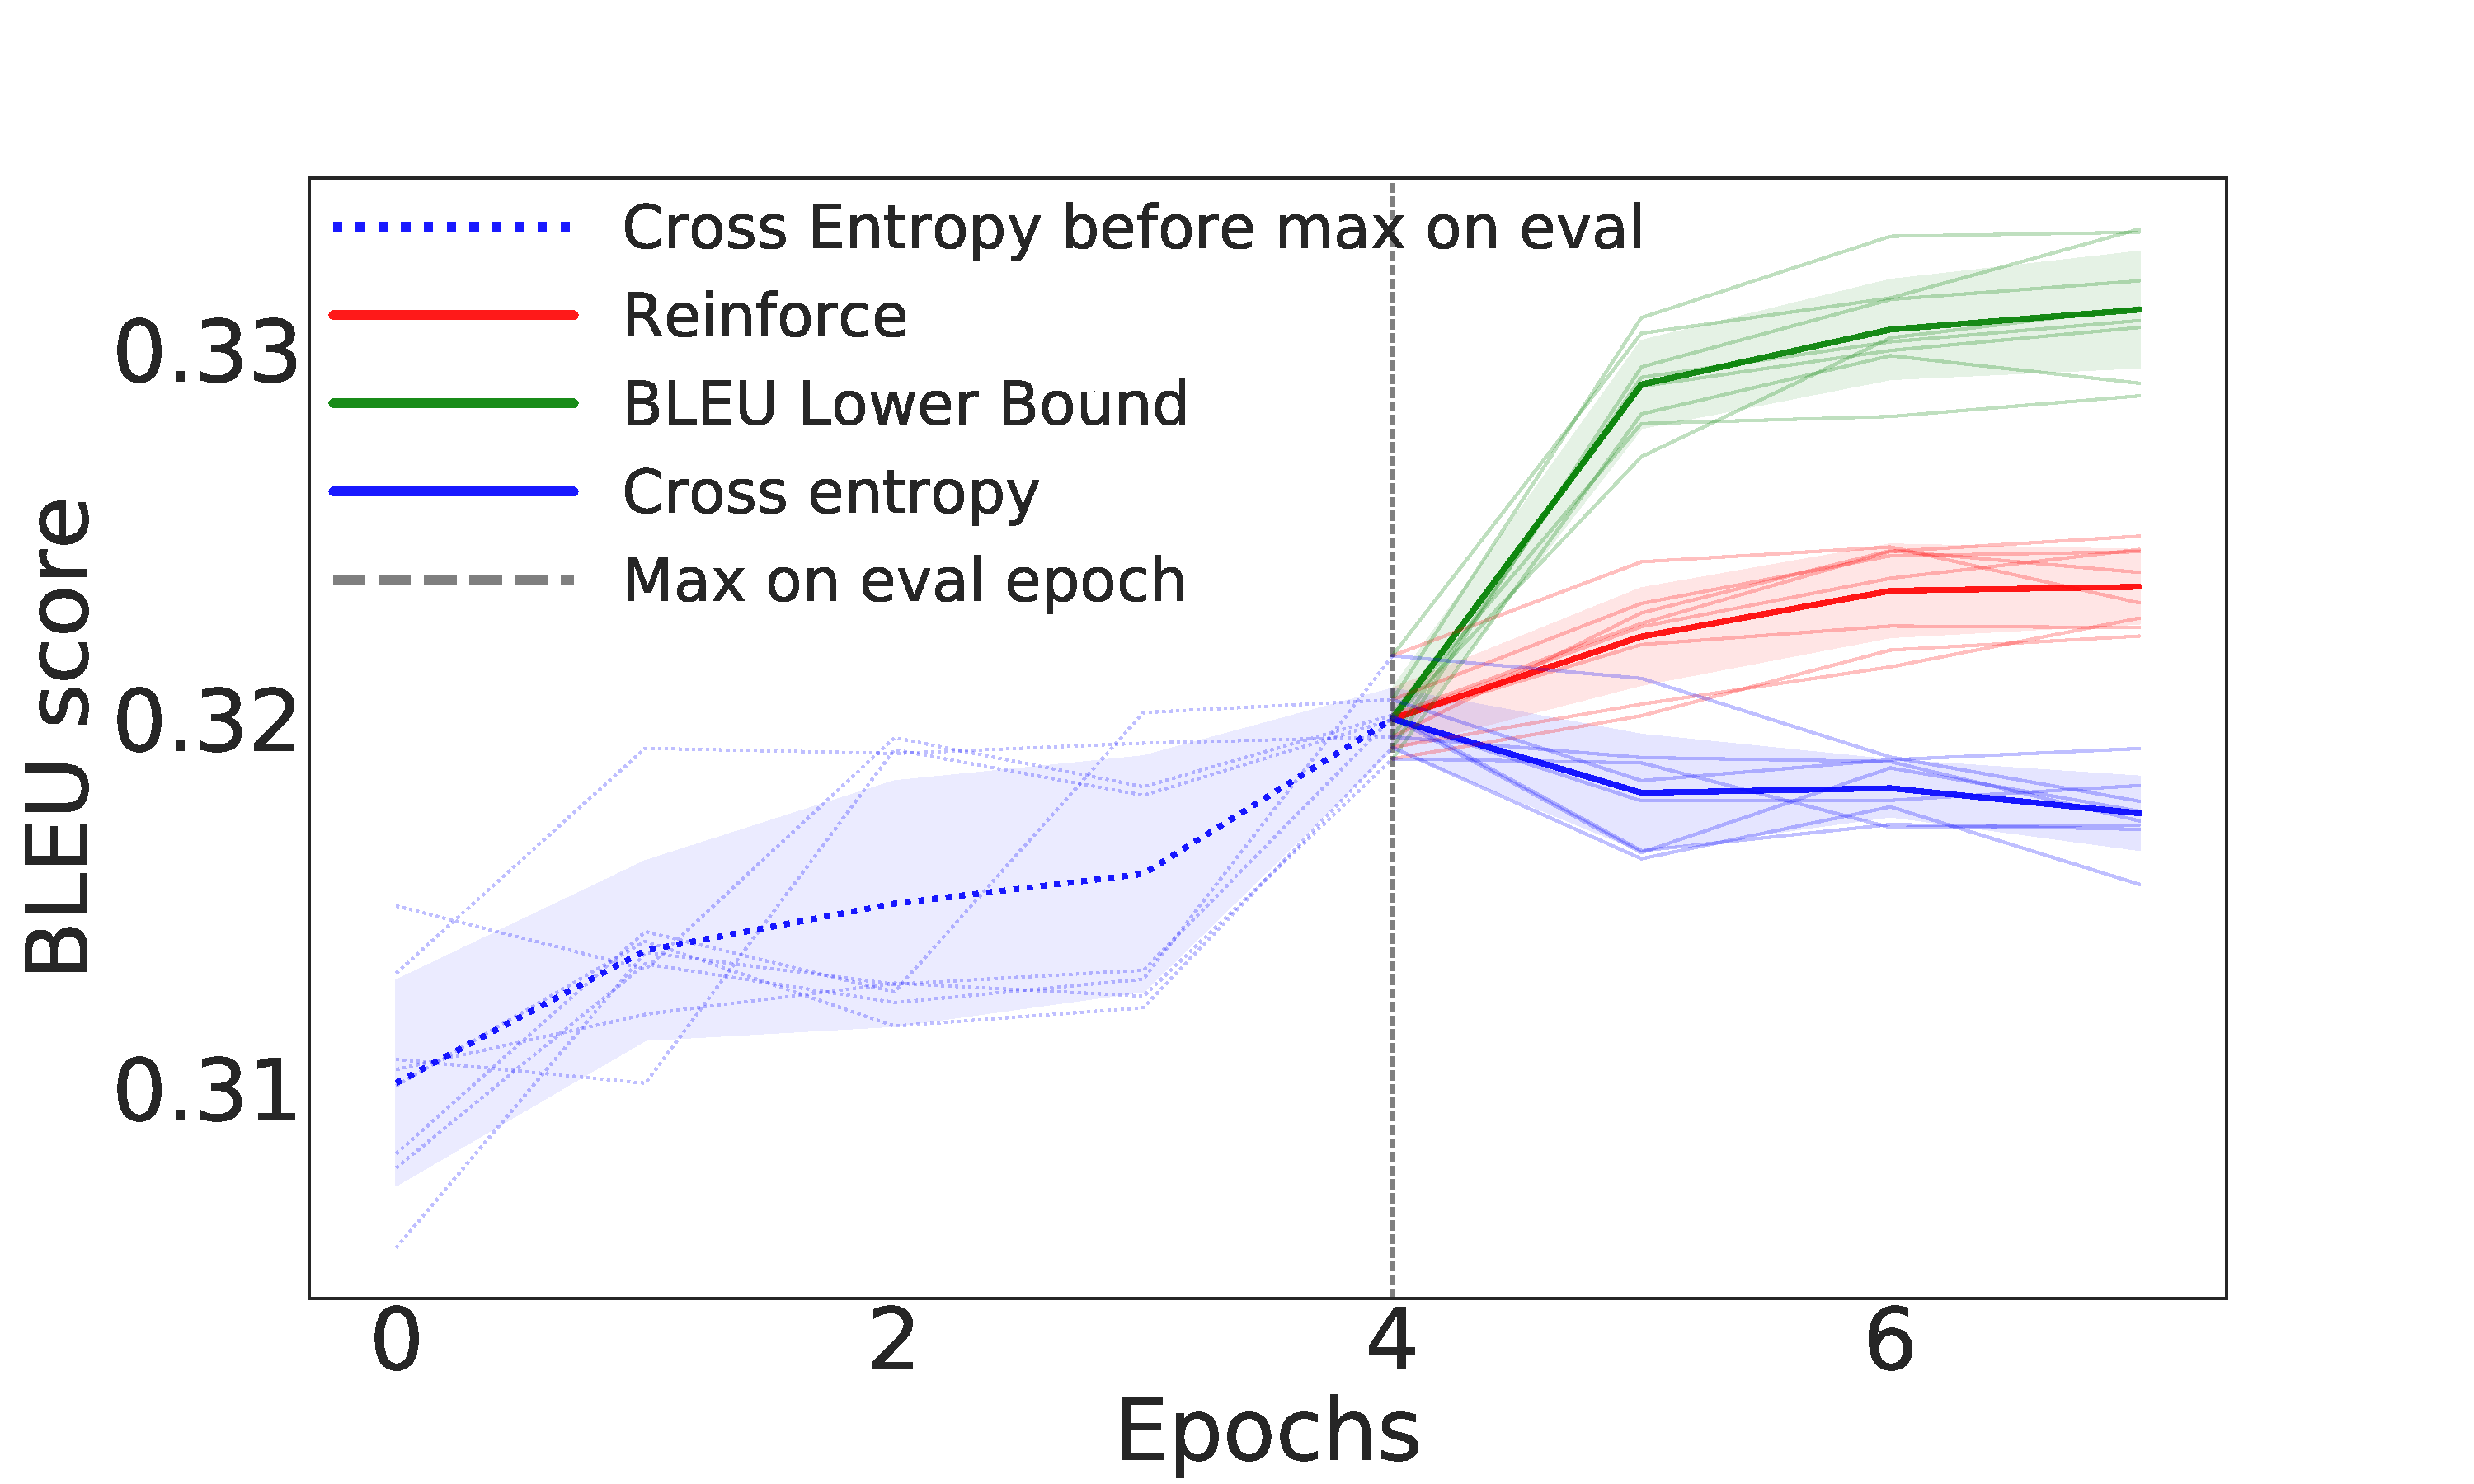
\includegraphics[scale=0.24]{res.pdf}
        \label{fig:results}
      \end{figure}
    \end{frame}

    \begin{frame}{Выводы}
        \begin{itemize}
            \item Эффективная, дифференцируемая нижняя оценка для математического ожидания метрики BLEU.
            \item Улучшение итоговой метрики на задаче перевода.
        \end{itemize}
    \end{frame}
    \begin{frame}{Возможное дальнейшее развитие}
        \begin{itemize}
            \item  Другие метрики:
            $$\mathbb{E}_{x\sim p_x,y\sim p_y} \lbrack  M(x, y) \rbrack=f(p_x, p_y)$$
            Аппроксимация математического ожидания произвольной метрики при помощи нейросетей.
            \item Добавление возможности оптимизации через стохастичность внутри сети:
            $$\mathbb{E}_{\mathrm{data}}\color{blue}{ \mathbb{E}_{\mathrm{arch\_stoch}}  \mathbb{E}_{\mathrm{output}} \textnormal{BLEU}(x, y) \to \max} $$
        \end{itemize}
    \end{frame}

    \begin{frame}{Вопросы}
        \Large{Вопросы?}
    \end{frame}

    \end{document}
    